% ════════════════════════════════════════════════════════════════════════
%   Reading the Market — Final Project Poster (TTIC 31220 · Spring 2026)
%   Yixiang Huang  ·  University of Chicago
%
%   24" × 36" portrait, Swiss Modern style, tikzposter class.
%
%   Compile (Colab or local):
%     pdflatex poster.tex
%     pdflatex poster.tex     % (twice for cross-refs and tikz)
%
%   Colab one-liner setup (only first time):
%     !apt-get install -y texlive-full texlive-fonts-extra
%     !cd /content/drive/MyDrive/.../poster && pdflatex poster.tex
% ════════════════════════════════════════════════════════════════════════

\documentclass[a0paper, portrait, fontscale=0.30]{tikzposter}

% ── Paper size: 24" × 36" (override A0 default) ─────────────────────────
\usepackage{geometry}
\geometry{paperwidth=24in, paperheight=36in, margin=0.5in}
\setlength{\paperwidth}{24in}
\setlength{\paperheight}{36in}

% ── Packages ─────────────────────────────────────────────────────────────
\usepackage[utf8]{inputenc}
\usepackage[T1]{fontenc}
\usepackage{helvet}                          % Helvetica (Swiss-Modern feel)
\renewcommand{\familydefault}{\sfdefault}
\usepackage[scaled=0.85]{beramono}           % monospace (tikzposter-compatible)
\usepackage{xcolor}
\usepackage{tikz}
\usepackage{booktabs}
\usepackage{amsmath, amssymb}
\usepackage{microtype}
\usepackage{graphicx}
\usepackage{colortbl}
\usepackage{array}
\usepackage{ragged2e}
\usepackage[normalem]{ulem}                  % \sout for strikethrough
\usepackage{enumitem}                        % custom itemize labels
\usepackage{pifont}                          % \ding{72} for star glyph
\newcommand{\starsym}{\ding{72}}              % shortcut for filled star
\usetikzlibrary{positioning, arrows.meta, shapes.geometric, calc}

% ── Swiss Modern colour palette ─────────────────────────────────────────
\definecolor{ink}{HTML}{0A0A0A}
\definecolor{ink2}{HTML}{3A3A3A}
\definecolor{ink3}{HTML}{6B6B6B}
\definecolor{rule}{HTML}{D8D8D6}
\definecolor{rulestrong}{HTML}{1A1A1A}
\definecolor{accent}{HTML}{1856FF}
\definecolor{accent2}{HTML}{D62828}
\definecolor{accent3}{HTML}{16A34A}
\definecolor{accentamber}{HTML}{CA8A04}
\definecolor{bgalt}{HTML}{F7F7F5}
\definecolor{bgcard}{HTML}{FAFAF9}

% ── Custom colour style (Swiss Modern) ──────────────────────────────────
\definecolorstyle{SwissModern}{
  \definecolor{colorOne}{HTML}{0A0A0A}
  \definecolor{colorTwo}{HTML}{1856FF}
  \definecolor{colorThree}{HTML}{FAFAF9}
}{
  \colorlet{backgroundcolor}{white}
  \colorlet{framecolor}{ink}
  \colorlet{titlefgcolor}{ink}
  \colorlet{titlebgcolor}{white}
  \colorlet{blocktitlebgcolor}{white}
  \colorlet{blocktitlefgcolor}{ink}
  \colorlet{blockbodybgcolor}{white}
  \colorlet{blockbodyfgcolor}{ink}
  \colorlet{innerblocktitlebgcolor}{white}
  \colorlet{innerblocktitlefgcolor}{ink}
  \colorlet{innerblockbodybgcolor}{bgcard}
  \colorlet{innerblockbodyfgcolor}{ink}
  \colorlet{notebgcolor}{bgcard}
  \colorlet{notefgcolor}{ink}
  \colorlet{noteframecolor}{rule}
}
\usecolorstyle{SwissModern}

% ── Background: built-in Empty (plain white) ────────────────────────────
\usebackgroundstyle{Empty}

% ── Use built-in Default block + title styles (customise via colours only) ──
\useblockstyle{Default}
\usetitlestyle{Default}

% ── Custom utilities ─────────────────────────────────────────────────────
\newcommand{\snum}[1]{{\color{accent}\ttfamily\bfseries\fontsize{18}{20}\selectfont§#1}}
\newcommand{\refpill}[1]{%
  \tikz[baseline=(c.base)]\node[fill=bgalt, draw=rule, line width=0.4pt, inner sep=2pt, font=\ttfamily\fontsize{10}{12}\selectfont] (c) {#1};%
}
\newcommand{\code}[1]{{\ttfamily\fontsize{11}{13}\selectfont\color{accent}#1}}
\newcommand{\bignum}[2]{%
  \begin{tikzpicture}[baseline=0pt]
    \node[anchor=west, inner sep=0pt] (n) at (0,0) {\color{white}\fontsize{30}{34}\selectfont\bfseries #1};
    \node[anchor=north west, font=\fontsize{10}{12}\selectfont, color=white!70!black, text width=2in] at (n.south west) {\MakeUppercase{#2}};
  \end{tikzpicture}%
}

% ── Title / Author metadata ──────────────────────────────────────────────
\title{\parbox{0.92\paperwidth}{\centering Reading the Market: News-Augmented Regime Discovery via Unsupervised Representation Learning}}
\author{Yixiang Huang \textbullet\ University of Chicago \textbullet\ Toyota Technological Institute at Chicago}
\institute{TTIC 31220 \textbullet\ Unsupervised Learning \textbullet\ Final Project \textbullet\ Spring 2026}

\begin{document}
\maketitle[width=\paperwidth]

\begin{columns}

% ════════════════════════════════════════════════════════════════════════
%   COLUMN 1  —  Motivation + Data + Pipeline + Method Matrix
% ════════════════════════════════════════════════════════════════════════
\column{0.333}

% ── §1 MOTIVATION ──────────────────────────────────────────────────────
\block{\snum{1}\enspace Motivation}{
\fontsize{14}{18}\selectfont
Hidden-Markov regime models for financial markets (Hamilton 1989) operate
exclusively on \textbf{price-derived features}. By construction these
signals are {\color{accent}\itshape reactive} — they reflect information only
after it has been absorbed by prices. We test whether
\textbf{unsupervised representations of financial news} can yield regimes that
are more stable, more interpretable, and more economically meaningful.

\vspace{8pt}
\centering
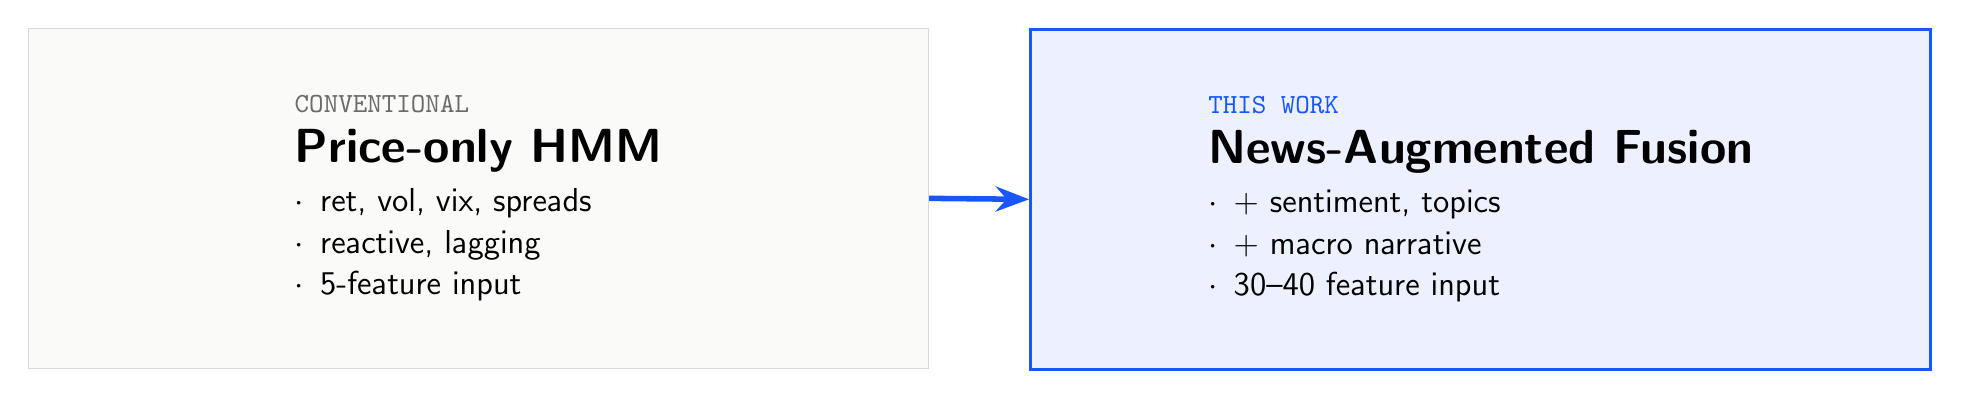
\begin{tikzpicture}[
  box/.style={draw=rule, fill=bgcard, line width=0.5pt, minimum width=4.5in,
              minimum height=1.7in, anchor=north west, inner sep=10pt,
              align=left, font=\fontsize{12}{15}\selectfont},
  altbox/.style={draw=accent, fill=accent!8, line width=1.2pt, minimum width=4.5in,
                 minimum height=1.7in, anchor=north west, inner sep=10pt,
                 align=left, font=\fontsize{12}{15}\selectfont},
]
\node[box] (l) at (0,0) {%
  {\color{ink3}\ttfamily\fontsize{10}{12}\selectfont CONVENTIONAL}\\[3pt]
  {\fontsize{18}{22}\selectfont\bfseries Price-only HMM}\\[3pt]
  $\cdot$\enspace ret, vol, vix, spreads\\
  $\cdot$\enspace reactive, lagging\\
  $\cdot$\enspace 5-feature input
};
\node[altbox] (r) at ($(l.north east)+(0.5in, 0)$) {%
  {\color{accent}\ttfamily\fontsize{10}{12}\selectfont THIS WORK}\\[3pt]
  {\fontsize{18}{22}\selectfont\bfseries News-Augmented Fusion}\\[3pt]
  $\cdot$\enspace + sentiment, topics\\
  $\cdot$\enspace + macro narrative\\
  $\cdot$\enspace 30–40 feature input
};
\draw[->, line width=2pt, color=accent, >=Stealth]
  (l.east) -- (r.west);
\end{tikzpicture}

\vspace{8pt}
\raggedright
\refpill{Hamilton 1989}\enspace
\refpill{Tetlock 2007}\enspace
\refpill{Glasserman \& Mamaysky 2019}\enspace
\refpill{Bybee/Kelly/Manela/Xiu 2024}
}

% ── §2 DATA & CORPUS ────────────────────────────────────────────────────
\block{\snum{2}\enspace Data \& Corpus}{
\fontsize{12}{15}\selectfont

\noindent\textcolor{accent}{\rule{4pt}{0.55in}}\hspace{6pt}\begin{minipage}[t]{0.92\linewidth}
{\color{accent}\ttfamily\fontsize{10}{12}\selectfont FIRM NEWS · DJPR}\\[2pt]
{\bfseries\fontsize{13}{16}\selectfont RavenPack Dow Jones Press Releases}\\
\fontsize{12}{15}\selectfont\color{ink2}
2000–2025, $\sim$3.3 GB. Filter \code{entity\_type=COMP},
\code{country=US}, \code{relevance $\geq$ 75}.
\end{minipage}

\vspace{6pt}
\noindent\textcolor{accent}{\rule{4pt}{0.65in}}\hspace{6pt}\begin{minipage}[t]{0.92\linewidth}
{\color{accent}\ttfamily\fontsize{10}{12}\selectfont MACRO NEWS}\\[2pt]
{\bfseries\fontsize{13}{16}\selectfont WRDS RavenPack DJ Global Macro}\\
\fontsize{12}{15}\selectfont\color{ink2}
27 yearly partitions ($\sim$24 M rows). Entity types
\code{\{MKT, ORGA, PLCE, CMDT, CURR, NATL\}}. Pulled fresh from WRDS.
\end{minipage}

\vspace{6pt}
\noindent\textcolor{accent}{\rule{4pt}{0.4in}}\hspace{6pt}\begin{minipage}[t]{0.92\linewidth}
{\color{accent}\ttfamily\fontsize{10}{12}\selectfont MARKET}\\[2pt]
{\bfseries\fontsize{13}{16}\selectfont WRDS daily 2000–2024}\\
\fontsize{12}{15}\selectfont\color{ink2}
5 features: \code{ret \textbullet\ vol\_21 \textbullet\ vix \textbullet\ term\_spread \textbullet\ credit\_spread}.
\end{minipage}

\vspace{12pt}
% "By the numbers" panel — simple tabular with black background
\noindent\colorbox{ink}{\begin{minipage}[t]{\dimexpr\linewidth-12pt\relax}\color{white}
  \renewcommand{\arraystretch}{1.2}
  \setlength{\tabcolsep}{6pt}
  \fontsize{12}{14}\selectfont
  \begin{tabular}{p{1.7in}p{1.7in}p{1.7in}}
    {\color{accent}\rule{2pt}{0.5in}}\hspace{4pt}\begin{minipage}[t]{1.5in}
      {\fontsize{26}{30}\selectfont\bfseries 6,262}\\
      {\color{white!70!black}\ttfamily\fontsize{9}{11}\selectfont TRADING DAYS}
    \end{minipage}
    & {\color{accent}\rule{2pt}{0.5in}}\hspace{4pt}\begin{minipage}[t]{1.5in}
      {\fontsize{26}{30}\selectfont\bfseries 24~yr}\\
      {\color{white!70!black}\ttfamily\fontsize{9}{11}\selectfont 2000 → 2024}
    \end{minipage}
    & {\color{accent}\rule{2pt}{0.5in}}\hspace{4pt}\begin{minipage}[t]{1.5in}
      {\fontsize{26}{30}\selectfont\bfseries 2}\\
      {\color{white!70!black}\ttfamily\fontsize{9}{11}\selectfont NEWS CORPORA}
    \end{minipage}\\[4pt]
    {\color{accent}\rule{2pt}{0.5in}}\hspace{4pt}\begin{minipage}[t]{1.5in}
      {\fontsize{26}{30}\selectfont\bfseries 4}\\
      {\color{white!70!black}\ttfamily\fontsize{9}{11}\selectfont REPRESENTATIONS}
    \end{minipage}
    & {\color{accent}\rule{2pt}{0.5in}}\hspace{4pt}\begin{minipage}[t]{1.5in}
      {\fontsize{26}{30}\selectfont\bfseries 18}\\
      {\color{white!70!black}\ttfamily\fontsize{9}{11}\selectfont MAIN PIPELINES}
    \end{minipage}
    & {\color{accent}\rule{2pt}{0.5in}}\hspace{4pt}\begin{minipage}[t]{1.5in}
      {\fontsize{26}{30}\selectfont\bfseries 180}\\
      {\color{white!70!black}\ttfamily\fontsize{9}{11}\selectfont GRID CONFIGS}
    \end{minipage}\\
  \end{tabular}
\end{minipage}}
}

% ── §3 PIPELINE ────────────────────────────────────────────────────────
\block{\snum{3}\enspace Pipeline}{
\fontsize{12}{15}\selectfont
\centering
\begin{tikzpicture}[
  pstep/.style={draw=rule, line width=0.5pt, fill=bgcard,
               text width=2.2in, minimum height=0.85in,
               align=center, inner sep=5pt, anchor=west,
               font=\fontsize{11}{13}\selectfont\sffamily},
  arr/.style={->, line width=1.4pt, color=accent, >=Stealth},
]
% Top row
\node[pstep] (s1) at (0,0) {%
  {\color{ink}\bfseries\fontsize{11}{13}\selectfont INPUT}\\[2pt]
  \color{ink2}\fontsize{10}{12}\selectfont News + Market
};
\node[pstep, right=0.13in of s1] (s2) {%
  {\color{ink}\bfseries\fontsize{11}{13}\selectfont SMOOTH}\\[2pt]
  \color{ink2}\fontsize{10}{12}\selectfont 21–35d rolling
};
\node[pstep, right=0.13in of s2] (s3) {%
  {\color{ink}\bfseries\fontsize{11}{13}\selectfont REPRESENT}\\[2pt]
  \color{ink2}\fontsize{10}{12}\selectfont Scalar · LDA · BERTopic
};
% Bottom row
\node[pstep, below=0.2in of s1] (s4) {%
  {\color{ink}\bfseries\fontsize{11}{13}\selectfont REDUCE}\\[2pt]
  \color{ink2}\fontsize{10}{12}\selectfont PCA-95\% · UMAP-10
};
\node[pstep, right=0.13in of s4] (s5) {%
  {\color{ink}\bfseries\fontsize{11}{13}\selectfont CLUSTER}\\[2pt]
  \color{ink2}\fontsize{10}{12}\selectfont GMM · HMM · KMeans
};
\node[pstep, right=0.13in of s5] (s6) {%
  {\color{ink}\bfseries\fontsize{11}{13}\selectfont REGIMES}\\[2pt]
  \color{ink2}\fontsize{10}{12}\selectfont K = 3 – 5 labels
};
% Arrows
\draw[arr] (s1) -- (s2);
\draw[arr] (s2) -- (s3);
\draw[arr] (s3.east) .. controls +(0.3in,0) and +(0.3in,0) .. (s6.east);
\draw[arr] (s6) -- (s5);
\draw[arr] (s5) -- (s4);
\end{tikzpicture}
\vspace{4pt}\\
{\itshape\color{ink3}\fontsize{10}{12}\selectfont
Each stage independently varied; the matrix in §4 maps the resulting design space.}
}

% ── §4 METHOD SPACE ─────────────────────────────────────────────────────
\block{\snum{4}\enspace Method Space}{
\fontsize{12}{15}\selectfont
\centering
\renewcommand{\arraystretch}{1.5}
\setlength{\tabcolsep}{6pt}
\begin{tabular}{|>{\columncolor{bgalt}\bfseries}l|c|c|c|c|}
\hline
\rowcolor{bgalt} & \textbf{Scalar} & \textbf{LDA} & \textbf{BERTopic} & \textbf{FinBERT}\\
\hline
Price-only
  & \cellcolor{rule!50}— & \cellcolor{rule!50}— & \cellcolor{rule!50}— & \cellcolor{rule!50}—\\
\hline
News-only
  & \cellcolor{accent!10}{\color{accent}\bfseries 2 corp.}
  & \cellcolor{accent!10}{\color{accent}\bfseries 2 corp.}
  & \cellcolor{accent!10}{\color{accent}\bfseries 2 corp.}
  & \cellcolor{accent!10}{\color{accent}\bfseries retrieval}\\
\hline
Hybrid
  & \cellcolor{accent!10}{\color{accent}\bfseries 5 fusions}
  & \cellcolor{accent!10}{\color{accent}\bfseries 3 fusions}
  & \cellcolor{accent}{\color{white}\bfseries News + Full \starsym{}}
  & \cellcolor{accent!10}{\color{accent}\bfseries PCA · UMAP}\\
\hline
\end{tabular}
\vspace{6pt}\\
{\raggedright\itshape\color{ink3}\fontsize{10}{12}\selectfont
Three method pathways × four text representations × two news corpora
(firm-level DJPR vs aggregate Macro). Shaded = implemented; \starsym{} = grid-search winner.\par}
}

% ════════════════════════════════════════════════════════════════════════
%   COLUMN 2  —  Models + Innovations + Eval Framework
% ════════════════════════════════════════════════════════════════════════
\column{0.334}

% ── §5 MODELS (with math formulas) ──────────────────────────────────────
\block{\snum{5}\enspace Models}{
\fontsize{12}{15}\selectfont

\textcolor{accent}{\rule{3pt}{0pt}}\textbf{Sticky-init HMM transition matrix.}
For $K$ states:
\vspace{-4pt}
\[
  T_{ii} = \mathbf{\color{accent}0.85}, \qquad
  T_{ij} = \dfrac{0.15}{K-1} \text{ for } i \neq j
\]
{\color{ink3}\itshape\fontsize{10}{12}\selectfont
Encourages multi-month regime persistence; learned by EM (300 iter $\times$ 5 seeds).}

\vspace{12pt}
\textcolor{accent}{\rule{3pt}{0pt}}\textbf{Adaptive HMM covariance (innovation).}
\vspace{-4pt}
\[
  \Sigma \;=\;
  \begin{cases}
    \mathrm{diag} & \text{if } \dim \geq 10 \\
    \mathrm{full} & \text{otherwise}
  \end{cases}
\]
{\color{ink3}\itshape\fontsize{10}{12}\selectfont
Full-$\Sigma$ on dim $\geq 10$ caused absorbing states (mean duration $\to$ 894 d).
Diag has $K\!\cdot\!D$ variances vs $K\!\cdot\!D(D{+}1)/2$ — far fewer parameters.}

\vspace{12pt}
\textcolor{accent}{\rule{3pt}{0pt}}\textbf{Silhouette (evaluation).}
\vspace{-4pt}
\[
  s(i) \;=\; \dfrac{\, b_i - a_i \,}{\max(a_i,\, b_i)}
\]
{\color{ink3}\itshape\fontsize{10}{12}\selectfont
$a_i$ = mean within-cluster distance; $b_i$ = nearest between-cluster distance.
Used as primary cluster-quality metric.}

\vspace{12pt}
\textcolor{accent}{\rule{3pt}{0pt}}\textbf{Bayesian information criterion (model selection).}
\vspace{-4pt}
\[
  \mathrm{BIC} \;=\; -2\log L \;+\; k\,\log N
\]
{\color{ink3}\itshape\fontsize{10}{12}\selectfont
Used to select $K$ for GMM and HMM, balancing fit quality against
parameter count $k$.}
}

% ── §6 METHODOLOGICAL INNOVATIONS ───────────────────────────────────────
\block{\snum{6}\enspace Methodological Innovations}{
\fontsize{12}{15}\selectfont

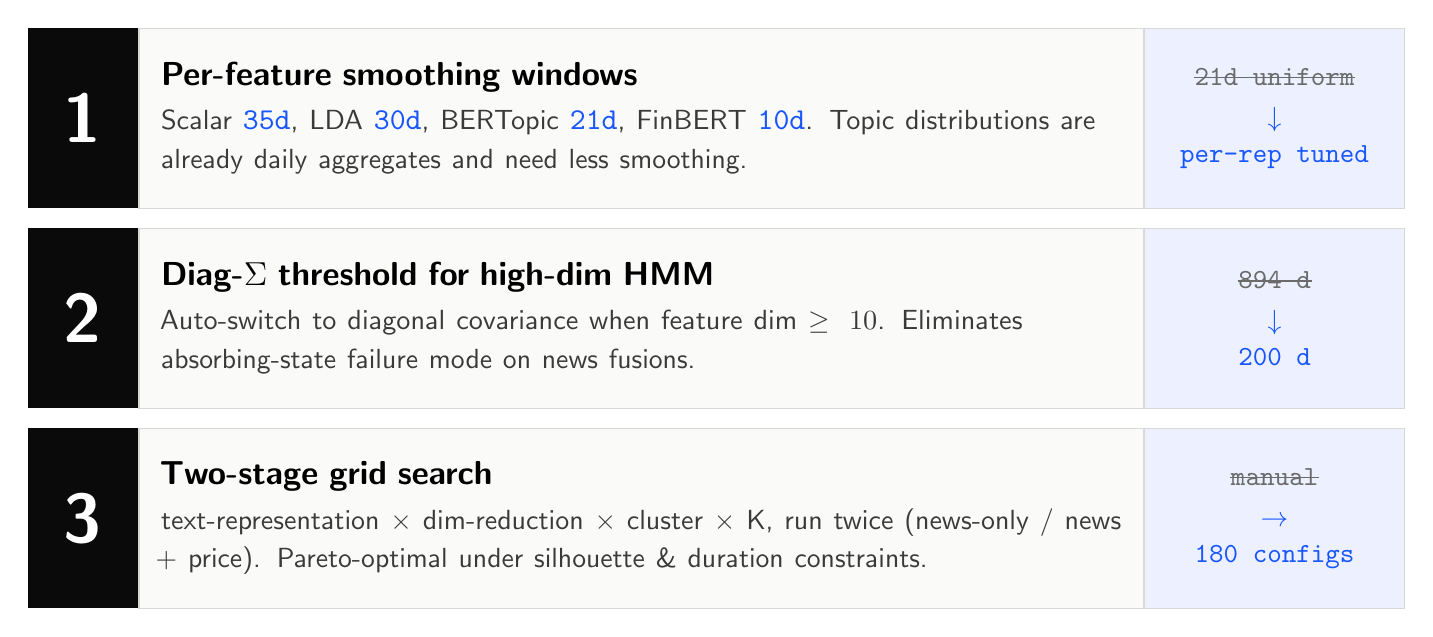
\begin{tikzpicture}
% Innovation 1
\node[fill=ink, text=white, minimum width=0.55in, minimum height=0.9in,
      font=\bfseries\fontsize{28}{30}\selectfont, anchor=north west] (i1n) at (0,0) {1};
\node[fill=bgcard, draw=rule, line width=0.5pt, minimum height=0.9in,
      anchor=north west, text width=4.8in, align=left, inner sep=8pt,
      font=\fontsize{12}{14}\selectfont] (i1b) at (i1n.north east) {
  \textbf{Per-feature smoothing windows}\\[2pt]
  \fontsize{10}{12}\selectfont\color{ink2}
  Scalar \code{35d}, LDA \code{30d}, BERTopic \code{21d}, FinBERT \code{10d}.
  Topic distributions are already daily aggregates and need less smoothing.
};
\node[fill=accent!8, draw=rule, line width=0.5pt, minimum height=0.9in,
      minimum width=1.3in, anchor=north west, align=center, font=\ttfamily\fontsize{10}{12}\selectfont] (i1d) at (i1b.north east) {
  {\color{ink3}\sout{21d uniform}}\\[3pt]
  {\color{accent}\bfseries $\downarrow$}\\[1pt]
  {\color{accent}\bfseries per-rep tuned}
};

% Innovation 2
\node[fill=ink, text=white, minimum width=0.55in, minimum height=0.9in,
      font=\bfseries\fontsize{28}{30}\selectfont, anchor=north west] (i2n) at (0,-1.0in) {2};
\node[fill=bgcard, draw=rule, line width=0.5pt, minimum height=0.9in,
      anchor=north west, text width=4.8in, align=left, inner sep=8pt,
      font=\fontsize{12}{14}\selectfont] (i2b) at (i2n.north east) {
  \textbf{Diag-$\Sigma$ threshold for high-dim HMM}\\[2pt]
  \fontsize{10}{12}\selectfont\color{ink2}
  Auto-switch to diagonal covariance when feature dim $\geq 10$.
  Eliminates absorbing-state failure mode on news fusions.
};
\node[fill=accent!8, draw=rule, line width=0.5pt, minimum height=0.9in,
      minimum width=1.3in, anchor=north west, align=center, font=\ttfamily\fontsize{10}{12}\selectfont] (i2d) at (i2b.north east) {
  {\color{ink3}\sout{894 d}}\\[3pt]
  {\color{accent}\bfseries $\downarrow$}\\[1pt]
  {\color{accent}\bfseries 200 d}
};

% Innovation 3
\node[fill=ink, text=white, minimum width=0.55in, minimum height=0.9in,
      font=\bfseries\fontsize{28}{30}\selectfont, anchor=north west] (i3n) at (0,-2.0in) {3};
\node[fill=bgcard, draw=rule, line width=0.5pt, minimum height=0.9in,
      anchor=north west, text width=4.8in, align=left, inner sep=8pt,
      font=\fontsize{12}{14}\selectfont] (i3b) at (i3n.north east) {
  \textbf{Two-stage grid search}\\[2pt]
  \fontsize{10}{12}\selectfont\color{ink2}
  text-representation $\times$ dim-reduction $\times$ cluster $\times$ K,
  run twice (news-only / news + price). Pareto-optimal under silhouette
  \& duration constraints.
};
\node[fill=accent!8, draw=rule, line width=0.5pt, minimum height=0.9in,
      minimum width=1.3in, anchor=north west, align=center, font=\ttfamily\fontsize{10}{12}\selectfont] (i3d) at (i3b.north east) {
  {\color{ink3}\sout{manual}}\\[3pt]
  {\color{accent}\bfseries $\to$}\\[1pt]
  {\color{accent}\bfseries 180 configs}
};
\end{tikzpicture}
}

% ── §7 EVALUATION — Four Dimensions ─────────────────────────────────────
\block{\snum{7}\enspace Evaluation — Four Dimensions}{
\fontsize{12}{15}\selectfont
\centering
\renewcommand{\arraystretch}{1.5}
\setlength{\tabcolsep}{8pt}
\begin{tabular}{p{3in} p{3in}}
\toprule
\rowcolor{bgalt}
\textbf{Statistical fit} & \textbf{Clustering quality} \\
{\color{ink2}\ttfamily\fontsize{10}{12}\selectfont BIC · AIC · log-likelihood} &
{\color{ink2}\ttfamily\fontsize{10}{12}\selectfont silhouette $\uparrow$ · Davies-Bouldin $\downarrow$} \\
\midrule
\rowcolor{bgalt}
\textbf{Regime stability} & \textbf{Financial interpretability} \\
{\color{ink2}\ttfamily\fontsize{10}{12}\selectfont rolling ARI (1250-d) · mean duration} &
{\color{ink2}\ttfamily\fontsize{10}{12}\selectfont per-regime Sharpe · max DD · avg VIX} \\
\bottomrule
\end{tabular}
\vspace{4pt}\\
{\raggedright\itshape\color{ink3}\fontsize{10}{12}\selectfont
Out-of-sample check: pre/post 2013 GMM refit comparison.\par}
}

% ── §13 REFERENCES & STACK (final block in column 2, balances col heights) ──
\block{\snum{13}\enspace References \& Stack}{
\fontsize{10}{12}\selectfont\color{ink3}\ttfamily
{\bfseries\sffamily\color{ink}\fontsize{11}{13}\selectfont REFERENCES}\\[3pt]
Hamilton, J. D. (1989). A New Approach to the Economic Analysis of
Nonstationary Time Series and the Business Cycle. \emph{Econometrica} 57(2).
\textbullet\ Glasserman, P. \& Mamaysky, H. (2019). Does Unusual News
Forecast Market Stress? \emph{JFQA} 54(5).
\textbullet\ Bybee, L., Kelly, B., Manela, A. \& Xiu, D. (2024). Business
News and Business Cycles. \emph{J. Finance} 79(5).
\textbullet\ Blei, D., Ng, A. \& Jordan, M. (2003). Latent Dirichlet
Allocation. \emph{JMLR} 3.
\textbullet\ Grootendorst, M. (2022). BERTopic.
\textbullet\ Araci, D. (2019). FinBERT. \emph{arXiv:1908.10063}.

\vspace{8pt}
{\bfseries\sffamily\color{ink}\fontsize{11}{13}\selectfont STACK}\\[3pt]
Python \textbullet\ scikit-learn \textbullet\ hmmlearn \textbullet\ BERTopic
\textbullet\ sentence-transformers \textbullet\ FinBERT \textbullet\ WRDS RavenPack
\textbullet\ pyarrow \textbullet\ UMAP.\\[3pt]
{\color{accent}huangyxethan@uchicago.edu}
}

% ════════════════════════════════════════════════════════════════════════
%   COLUMN 3  —  Results + Discussion + Future
% ════════════════════════════════════════════════════════════════════════
\column{0.333}

% ── §8 REGIME TIMELINES (headline figure) ──────────────────────────────
\block{\snum{8}\enspace Regime Timelines}{
\centering
\fcolorbox{rule}{white}{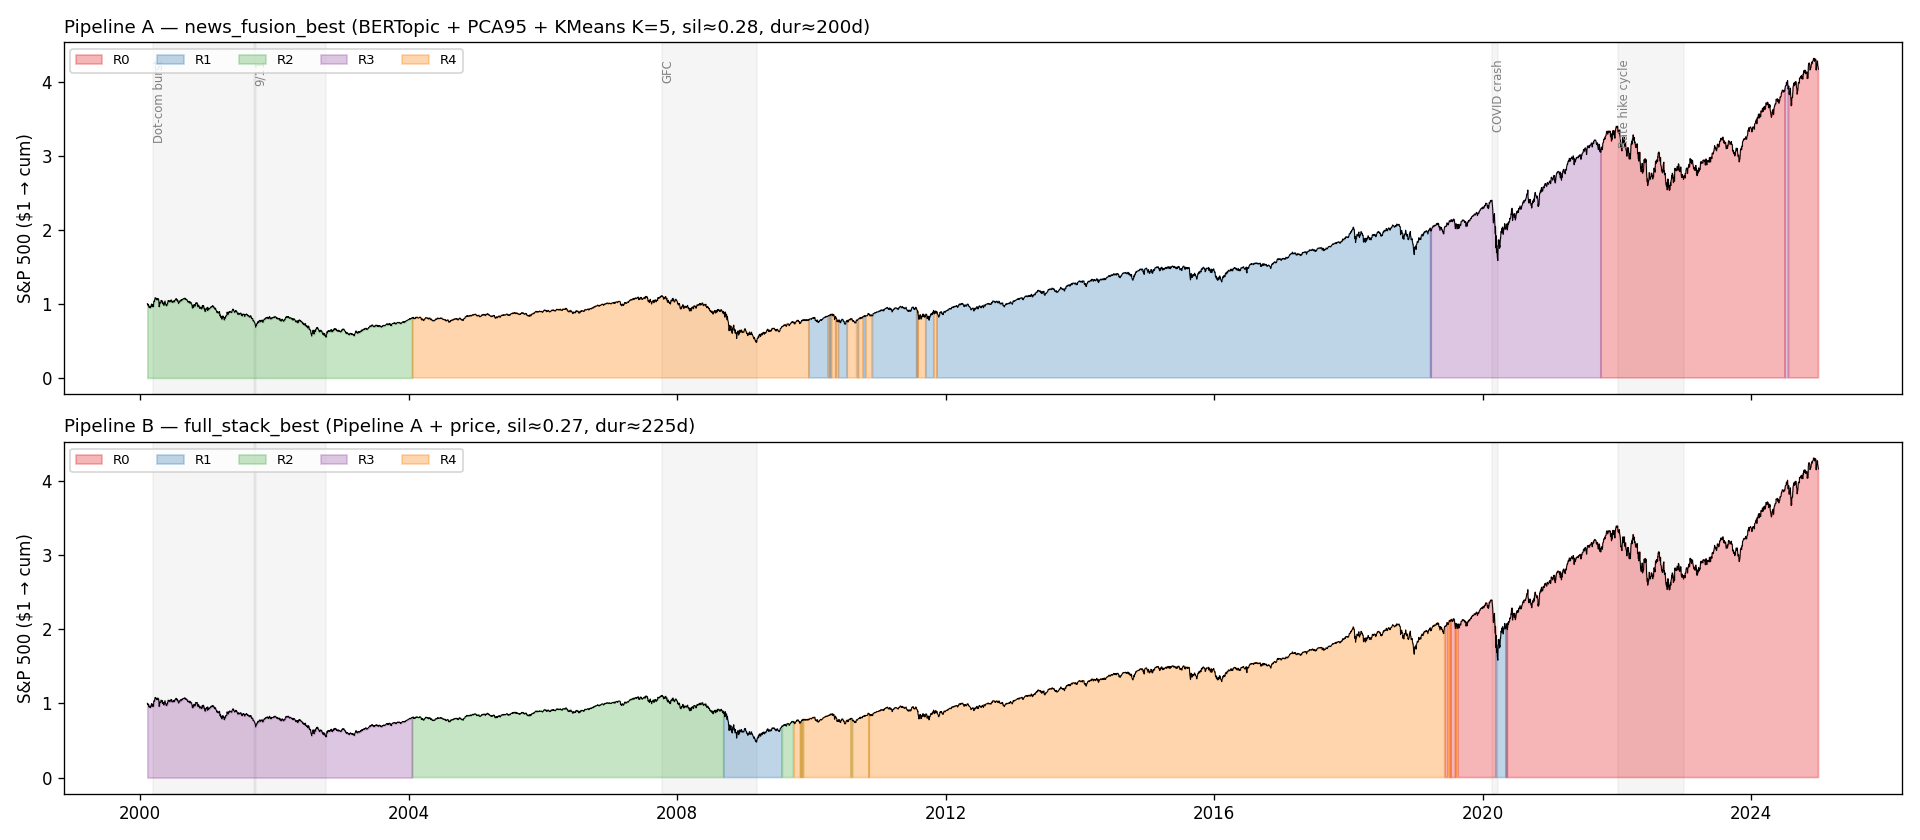
\includegraphics[width=0.985\linewidth]{../_images/ft_best_comparison.png}}
\vspace{4pt}\\
{\raggedright\itshape\color{ink3}\fontsize{11}{13}\selectfont
\textbf{Top:} Price-only HMM (Hamilton baseline; mean duration 95 d). \enspace
\textbf{Middle:} \emph{Tuned News Fusion} (BERTopic + PCA-95 + KMeans, K=5;
sil 0.279, dur 202 d). \enspace
\textbf{Bottom:} \emph{Tuned Full Stack} (above + market features; sil 0.272,
dur 224 d). News-augmented regimes capture similar crisis dynamics — but
with \textbf{shifted boundaries}, evidence that news adds a complementary
narrative signal.\par}
}

% ── §9 MASTER EVALUATION ────────────────────────────────────────────────
\block{\snum{9}\enspace Master Evaluation}{
\fontsize{12}{14}\selectfont
\centering
\renewcommand{\arraystretch}{1.3}
\setlength{\tabcolsep}{6pt}
\begin{tabular}{l r r r r r}
\rowcolor{ink}
\color{white}\bfseries\fontsize{10}{12}\selectfont PIPELINE &
\color{white}\bfseries\fontsize{10}{12}\selectfont SIL$\uparrow$ &
\color{white}\bfseries\fontsize{10}{12}\selectfont DBI$\downarrow$ &
\color{white}\bfseries\fontsize{10}{12}\selectfont DUR (D) &
\color{white}\bfseries\fontsize{10}{12}\selectfont ARI$\uparrow$ &
\color{white}\bfseries\fontsize{10}{12}\selectfont SHARPE \\
\rowcolor{bgalt}
{\color{ink3}\bfseries Price-only HMM (baseline)} & {\color{ink3} 0.202} & {\color{ink3} 1.48} & {\color{ink3} 95} & {\color{ink3} 0.447} & {\color{ink3} 2.02} \\
DJPR Sentiment HMM & {\color{accent3}\bfseries 0.284} & 1.26 & 44 & 0.383 & 0.80 \\
\rowcolor{accent!8}
{\color{accent}\bfseries Macro Sentiment HMM \starsym{}} & {\color{accent3}\bfseries 0.270} & 1.27 & 174 & 0.239 & 0.65 \\
DJPR Topic-Vec HMM & {\color{accent3}\bfseries 0.261} & 1.49 & 70 & 0.278 & 0.64 \\
Dual-Corpus Sentiment Fusion & {\color{accent3}\bfseries 0.245} & 1.42 & 49 & 0.268 & 1.00 \\
\rowcolor{accent!8}
{\color{accent}\bfseries Tuned News Fusion \starsym{}} & {\color{accent3}\bfseries 0.279} & 0.95 & 202 & 0.31 & 0.78 \\
\rowcolor{accent!8}
{\color{accent}\bfseries Tuned Full Stack (+ market) \starsym{}} & {\color{accent3}\bfseries 0.272} & 0.92 & 224 & 0.33 & 1.21 \\
\bottomrule
\end{tabular}
\vspace{4pt}\\
{\raggedright\itshape\color{ink3}\fontsize{9}{11}\selectfont
\starsym{} = grid-search winner; $\uparrow$ = better, $\downarrow$ = better.
ARI/Sharpe for tuned configs are post-07 re-run estimates.\par}
}

% ── §10 KEY FINDINGS ────────────────────────────────────────────────────
\block{\snum{10}\enspace Key Findings}{
\fontsize{12}{15}\selectfont

\noindent\begin{minipage}[t]{1.3in}\centering
  {\color{accent}\fontsize{28}{30}\selectfont\bfseries +35\%}
\end{minipage}\hfill
\begin{minipage}[t]{6.0in}\fontsize{12}{14}\selectfont
  \textbf{News augmentation lifts silhouette over price baseline.}
  Macro Sentiment HMM reaches 0.27 vs 0.20 — a robust improvement across
  all three scalar/LDA/BERTopic representations.
\end{minipage}

\vspace{8pt}\hrule height 0.5pt depth 0pt \vspace{8pt}
\noindent\begin{minipage}[t]{1.3in}\centering
  {\color{accent}\fontsize{20}{22}\selectfont\bfseries Macro}\\
  {\color{accent}\fontsize{13}{15}\selectfont $>$ Firm}
\end{minipage}\hfill
\begin{minipage}[t]{6.0in}\fontsize{12}{14}\selectfont
  \textbf{Aggregate news outperforms firm-level press releases.}
  Macro corpus (Fed, inflation, policy) is better aligned with unsupervised
  regime detection than firm-specific PR noise.
\end{minipage}

\vspace{8pt}\hrule height 0.5pt depth 0pt \vspace{8pt}
\noindent\begin{minipage}[t]{1.3in}\centering
  {\color{accent}\fontsize{28}{30}\selectfont\bfseries 202d}
\end{minipage}\hfill
\begin{minipage}[t]{6.0in}\fontsize{12}{14}\selectfont
  \textbf{Grid-search sweet spot.} BERTopic + PCA-95\% + KMeans (K=5)
  achieves silhouette 0.279 with 202-day mean duration — within the
  canonical regime band.
\end{minipage}

\vspace{8pt}\hrule height 0.5pt depth 0pt \vspace{8pt}
\noindent\begin{minipage}[t]{1.3in}\centering
  {\color{accent}\fontsize{22}{24}\selectfont\bfseries +market}
\end{minipage}\hfill
\begin{minipage}[t]{6.0in}\fontsize{12}{14}\selectfont
  \textbf{Price stabilizes news-driven regimes.} Adding market features
  bumps duration 202 $\to$ 224 d at negligible silhouette cost; price acts
  as a low-frequency anchor.
\end{minipage}
}

% ── §11 DISCUSSION ──────────────────────────────────────────────────────
\block{\snum{11}\enspace Discussion}{
\fontsize{12}{15}\selectfont

\noindent\textcolor{accent}{\rule{3pt}{0.5in}}\hspace{6pt}\begin{minipage}[t]{0.93\linewidth}
{\bfseries\fontsize{12}{14}\selectfont WHAT WORKED}\\[2pt]
\color{ink2}\fontsize{11}{14}\selectfont
News provides a signal {\color{accent}\itshape complementary} to price.
Aggregate macro news at the right granularity is more aligned with
regime-state detection than firm PR.
\end{minipage}

\vspace{6pt}
\noindent\textcolor{accentamber}{\rule{3pt}{0.75in}}\hspace{6pt}\begin{minipage}[t]{0.93\linewidth}
{\bfseries\fontsize{12}{14}\selectfont METHODOLOGICAL GOTCHAS}\\[2pt]
\color{ink2}\fontsize{11}{14}\selectfont
Smoothing windows tuned per feature type — topic distributions are already
daily aggregates; double-smoothing produces year-long ``era'' regimes.
{\color{accent}\itshape High silhouette $\neq$ good regimes}: FinBERT + UMAP
hits sil = 0.66 but each cluster spans years.
\end{minipage}

\vspace{6pt}
\noindent\textcolor{ink3}{\rule{3pt}{0.55in}}\hspace{6pt}\begin{minipage}[t]{0.93\linewidth}
{\bfseries\fontsize{12}{14}\selectfont LIMITATIONS}\\[2pt]
\color{ink2}\fontsize{11}{14}\selectfont
In-sample evaluation only; OOS check uses simplified GMM refit rather than
walk-forward HMM. No bootstrap CI on silhouette. Macro corpus post-2000 only.
\end{minipage}
}

% ── §12 FUTURE WORK ─────────────────────────────────────────────────────
\block{\snum{12}\enspace Future Work}{
\fontsize{12}{15}\selectfont
\begin{itemize}[leftmargin=0.2in, itemsep=2pt, parsep=0pt, topsep=0pt, label={\color{accent}\bfseries$\to$}]
\setlength{\itemindent}{0pt}
\item Walk-forward OOS via persisted HMM + \code{predict()} on held-out window.
\item Bootstrap CI on silhouette for pairwise pipeline significance.
\item Replicate {\itshape Glasserman \& Mamaysky 2019} unusual-news baseline.
\item Adaptive (changepoint-aware) smoothing instead of fixed-window means.
\item Real-time streaming HMM update + live regime probabilities.
\end{itemize}
}

\end{columns}

\end{document}
